\documentclass[aspectratio=169,10pt,xcolor={dvipsnames}]{beamer}
\usetheme[
%%% option passed to the outer theme
%    progressstyle=fixedCircCnt,   % fixedCircCnt, movingCircCnt (moving is deault)
  ]{Cores}
  
% If you want to change the colors of the various elements in the theme, edit and uncomment the following lines

% Change the bar colors:
\setbeamercolor{Feather}{fg=redCORES,bg=white}

% Change the color of the structural elements:
\setbeamercolor{structure}{fg=red}

% Change the frame title text color:
\setbeamercolor{frametitle}{fg=darkgray}

% Change the normal text colors:
\setbeamercolor{normal text}{fg=black!75,bg=gray!5}

%% Change the block title colors
% \setbeamercolor{block title}{use=Feather,bg=Feather.fg, fg=black!90} 
\setbeamercolor{block title}{fg=black,bg=redCORES}
\setbeamercolor{title}{fg=white}
\setbeamercolor{author}{fg=gray}
\setbeamercolor{institute}{fg=gray}


% Change the logo in the upper right circle:
%\renewcommand{\logofile}{example-grid-100x100pt} 
%% This is an image that comes with the LaTeX installation
% Adjust scale of the logo w.r.t. the circle; default is 0.875
\renewcommand{\logoscale}{1}

% Change the background image on the title and final page.
% It stretches to fill the entire frame!
% \renewcommand{\backgroundfile}{example-grid-100x100pt}

%-------------------------------------------------------
% INCLUDE PACKAGES
%-------------------------------------------------------
\usepackage{helvet}
\usepackage[absolute,overlay]{textpos}

\usepackage[utf8]{inputenc}
% \usepackage[english]{babel}
\usepackage[portuguese]{babel}
\usepackage[T1]{fontenc}
\usepackage{helvet}

%% Load different font packages to use different fonts
%% e.g. using Linux Libertine, Linux Biolinum and Inconsolata
% \usepackage{libertine}
% \usepackage{zi4}

%% e.g. using Carlito and Caladea
% \usepackage{carlito}
% \usepackage{caladea}
% \usepackage{zi4}

%% e.g. using Venturis ADF Serif and Sans
% \usepackage{venturis}

%-------------------------------------------------------
% DEFFINING AND REDEFINING COMMANDS
%-------------------------------------------------------

% colored hyperlinks
\newcommand{\chref}[2]{
  \href{#1}{{\usebeamercolor[bg]{Feather}#2}}
}

%-------------------------------------------------------

% INFORMATION IN THE TITLE PAGE
%-------------------------------------------------------

\title[Aplicando DSR na identificação de Sintomas de Depressão em Mídias Sociais] % [] is optional - is placed on the bottom of the sidebar on every slide
{ % is placed on the title page
      \Large{\textbf{Aplicando DSR na identificação de }\\ 
      \textbf{Sintomas de Depressão em Mídias Sociais}}
% \hspace*{5pt} 
}

\subtitle[]
{
      \textbf{}
}

\author[Silas P. Lima Filho]
{      {Silas P. Lima Filho \hspace{50pt} Monica F. da Silva \hspace{50pt} Jonice Oliveira}\\
      {\ttfamily \hspace*{-10pt}silaslfilho@ppgi.ufrj.br \hspace{12pt} monica@ppgi.ufrj.br  \hspace{25pt}jonice@dcc.ufrj.br}
}

\institute[]
{%
      Programa de Pós-Graduação em Informática\\
      Instituto de Matemática\\
      Universidade Federal do Rio de Janeiro
}

\date{\today}

%-------------------------------------------------------
% THE BODY OF THE PRESENTATION
%-------------------------------------------------------

\begin{document}

{
\definecolor{backgroundcolor}{RGB}{30,30,30} % msm cor do layout atual
\definecolor{text}{RGB}{255,255,255}
\setbeamercolor{background canvas}{bg=backgroundcolor}
    \begin{frame}[plain,noframenumbering]
        % Definicao da posicao da logo ufrj
        \begin{textblock*}{\textwidth}(.5cm, .5cm)
             
\includegraphics[scale=.1]{./Graphics/minervaNEW.png}
        \end{textblock*}
 
        % Definicao da posicao da logo cores
        \begin{textblock*}{\textwidth}(10.5cm, .6cm)
            
\includegraphics[scale=.225]{./Graphics/logo_lab_fundopreto.png}
        \end{textblock*}

        \vspace*{-.2cm}
        \hspace*{-.5cm}
        \begin{textblock*}{\textwidth}(.3cm, 3.8cm)
            {\usebeamercolor[fg]{titlegraphic}\inserttitlegraphic\par}
            \begin{beamercolorbox}[sep=8pt, 
                                   left, 
                                  colsep=-4bp, 
                                  rounded=true, 
                                  shadow=true]{title}
            % \usebeamerfont{title}
            \inserttitle
            \par%
                \ifx
                    \insertsubtitle
                    \@empty%
                    \else%
                    \vskip0.18cm%
                    \hspace{.4cm}
                    {\usebeamerfont{subtitle}\usebeamercolor[fg]{subtitle}
                    \insertsubtitle
                    \par}%
                \fi%     
            \end{beamercolorbox}%

            \vskip1em\par

            \begin{beamercolorbox}[sep=8pt, left,colsep=-4bp,rounded=true,shadow=true]{author}
               \usebeamerfont{author}
               \insertauthor
            \end{beamercolorbox}

    	    \begin{beamercolorbox}[sep=8pt,center,colsep=-4bp,rounded=true,shadow=true]{institute}
               \usebeamerfont{institute}
               \insertinstitute
            \end{beamercolorbox}

            %  \begin{beamercolorbox}[sep=8pt,center,colsep=-4bp,rounded=true,shadow=true]{date}
            %     % \usebeamerfont{date}
            %     \insertdate
            %  \end{beamercolorbox}%\vskip0.5em
        \end{textblock*}
      %\titlepage
    \end{frame}}

%-------------------------------------------------------
% THE TITLEPAGE
%-------------------------------------------------------

% {\1% % this is the name of the PDF file for the background
% \begin{frame}[plain,noframenumbering] % the plain option removes the header from the title page, noframenumbering removes the numbering of this frame only
%   \titlepage % call the title page information from above
% \end{frame}}


% \begin{frame}{Content}{}
% \tableofcontents
% \end{frame}

%-------------------------------------------------------


% \begin{frame}{Referencial de DSR}
%   \begin{block}{}
%     Segundo Peffers\cite{Peffers2007}: "This process is structured in a nominally sequential order; however, there is no expectation that researchers would always proceed in sequential order from activity 1 through activity 6. In reality, they may actually start at almost any step and move outward. A problem-centered approach is the basis of the nominal sequence, starting with activity 1. Researchers might proceed in this sequence if the idea for the research resulted from observation of the problem or from suggested future research in a paper from a prior project. An objective-centered solution, starting with activity 2, could be triggered by an industry or research need that can be addressed by developing an artifact. A design- and development-centered approach would start with activity 3. It would result from the existence of an artifact that has not yet been formally thought through as a solution for the explicit problem domain in which it will be used."
%   \end{block}
% \end{frame}


\section{Referencial de DSR}
\begin{frame}{Referencial}
  \begin{figure}
    \centering
    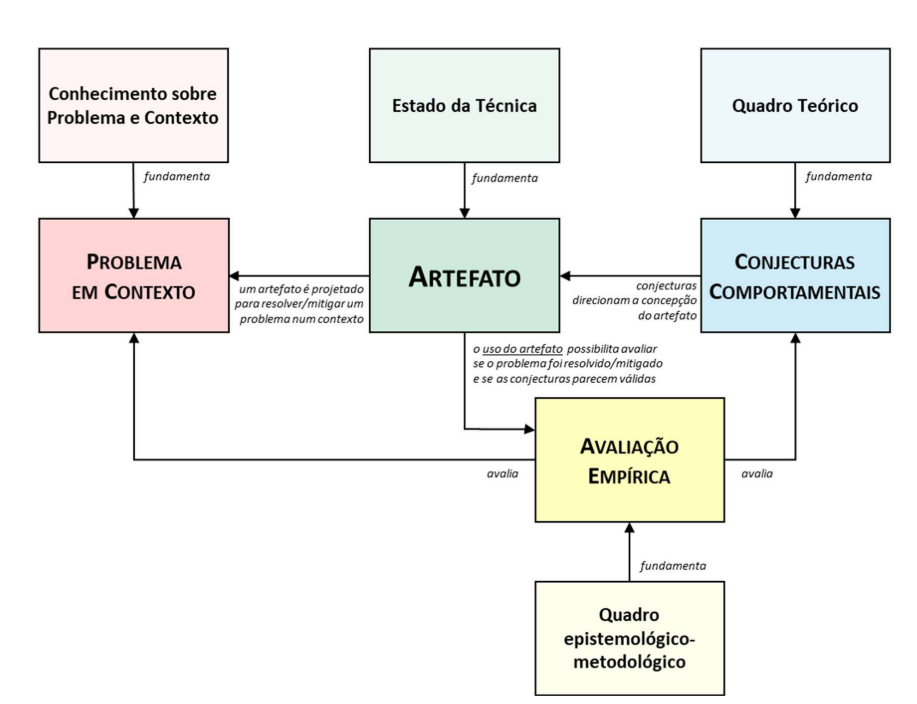
\includegraphics[scale=.25]{Graphics/Pimentel_DSR_Model.png}
    \caption{Modelo DSR proposto por \cite{Pimentel2020}.}
  \end{figure}
\end{frame}

\section{Estrutura da Pesquisa}
\begin{frame}{Estrutura da Pesquisa}{}
  \textbf{\large Contexto}

  \begin{block}{}
    Saúde mental tem sido discutida em diferentes círculos sociais e diferentes mídias. Infelizmente, diferentes grupos sociais, econômicos e étnicos são afetados pela falta de cuidados e tratamento de saúde mental. Depressão é uma das doenças mentais mais relacionadas no mundo. Com a disseminação e com mais pessoas com depressão, torna-se um desafio identificar uma pessoa, ou população que pode estar em um estado real de depressão.
  \end{block}
\end{frame}

\begin{frame}{Estrutura da Pesquisa}{}
  \textbf{\large Problema e Caracterização}

  \begin{block}{}
    \begin{itemize}
      \item Uma vez que o conhecimento da revisão da literatura tem apresentado uma fraca colaboração entre a informática e a psicologia, destaca-se que nem sempre é levado em consideração como profissionais inferem se alguém é depressivo ou não. Como um dos sintomas da depressão é a inatividade, um usuário depressivo pode não gerar conteúdo online de forma consistente. 
    
      \item Como o contexto da psicologia lida regularmente com a subjetividade da informação, espera-se que informações relevantes podem ser extraídas de outros métodos, em vez de apenas conteúdo textual. Acreditamos que a classificação de potenciais usuários depressivos poderia ser mais confiável se combinada com ``informações subjetivas''.
    \end{itemize}
  \end{block}

  % \begin{block}{}
  %   Uma vez que o conhecimento da revisão da literatura tem apresentado uma fraca colaboração entre a informática e a psicologia, as contribuições esperadas estão relacionadas a essas duas áreas de pesquisa. Para criar um artefato útil, enfrenta diferentes estágios que podem oferecer desafios de pesquisa a serem realizados. Como o produto final é a habilidade de identificar sintomas de depressão, devemos passar por etapas como obter, processar, modelar e persistir os dados de sites de redes sociais em uma estrutura que possa permitir as próximas etapas para recuperar esses dados para análises futuras. Nosso método visa identificar um usuário depressivo inserido em uma rede social de forma confiável, consistente e discreta.
  % \end{block}
\end{frame}


\begin{frame}{Estrutura da Pesquisa}{}
  
  \textbf{\large Conjecturas Teóricas}
  
  \begin{block}{}
    \begin{itemize}
      \item Revisão Literatura - Busca por conceitos e construtos relacionados ao contexto.
      \item Revisão Sistemática da Literatura - Busca pelo atual estado da arte.
    \end{itemize}
  \end{block}
  % \normalsize
  \begin{block}{}
    \begin{itemize}
      \item[\textbullet] Análise de Redes Sociais - Técnicas de monitoramento
      \item[\textbullet] Conceitos Depressão - \cite{american2013diagnostic}
      \item[\textbullet] Reconhecimento de Padrões - \cite{Nolasco2016}
    \end{itemize}
  \end{block}
    % Após uma primeira iteração utilizando revisão sistemática da literatura, selecionamos artigos com contribuições na área de inteligência artificial, especificamente em soluções de aprendizado de máquina e deep learning. Destes trabalhos, podemos extrair diferentes abordagens como: identificar quais sintomas são encontrados nas redes sociais e irão compor um modelo como features; criação de um modelo de classificação de um potencial depressivo.
   
    % Com as contribuições identificadas na literatura, extraímos os recursos utilizados nesses trabalhos. Com uma espécie de investigação em soluções computacionais para a identificação prévia de grupos populacionais depressivos, é intrigante saber se essas contribuições são de fato práticas para especialistas no domínio. Não apenas prático, mas se as informações e dados empregados são relevantes em um cenário real de diagnóstico clínico de depressão.

    % O problema de lidar com a depressão e as redes sociais pode ser entendido como uma busca por pessoas que sofrem os sintomas da depressão.
  
    
\end{frame}

\begin{frame}{Estrutura da Pesquisa}{}

  \textbf{\large Artefato}
  \begin{block}{}
    Criação de um modelo de classificação que leve em consideração não apenas características textuais, mas também subjetivas (temporais, comunidade e comportamentais). Propondo assim uma maior aproximação de uma identificação feita por um profissional.
  \end{block}
  
  \textbf{\large Estado da Técnica}
  \begin{block}{}
      \begin{itemize}
        \item Uso de características textuais - LIWC
        \item Redes Neurais Recorrentes
        \item Refinamento(fine-tuning) de modelos
      \end{itemize}
  \end{block}
\end{frame}


\begin{frame}{Estrutura da Pesquisa}

  \textbf{\large Avaliações*}
  \begin{block}{Reaproveitamento das Perguntas de Pesquisa da RSL}
    \begin{itemize}
      \item Seria possivel identificar sintomas de doencas psicologicas por meio das midias sociais? 
      \item Haveria uma forma de diagnosticar um distúrbio usando apenas informacoes das MS? 	
      \item Seriam as MS's uteis para profissionais, psicologos etc? 	
      \item Que tipos de tecnicas de analise poderiam ser utilizadas para tal? 	
      \item Quais são os trabalhos existentes atuais que abordam depressão? 	
      \item Quando e onde os trabalhos tem sido publicados? 	
      \item Quão próximos da realidade um modelo de classificação pode ser? 
    \end{itemize}
  
  \end{block}
\end{frame}  


\begin{frame}{Estrutura da Pesquisa}

  \textbf{\large Avaliações*}
  \begin{block}{}
    \begin{itemize}
      \item Estudo de caso com 3 psicólogos,
      \item Survey com 49 profissionais da saúde
    \end{itemize}
  \end{block}
\end{frame}  
  % \begin{block}{Resultados}
    
  % \end{block}

\begin{frame}{Estrutura da Pesquisa}
  \textbf{\large Publicações}
  \begin{block}{}
    \begin{itemize}
      \item WTDBD 2020
    \end{itemize}
  \end{block}
\end{frame}


\begin{frame}
  \begin{figure}
    \centering
    % 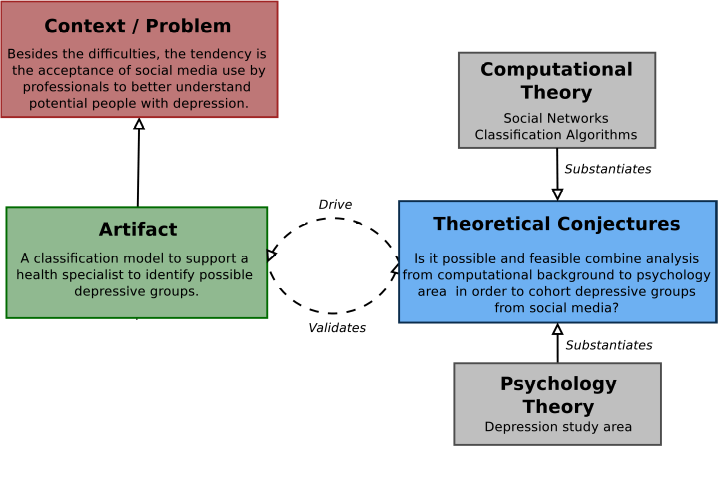
\includegraphics[scale=.4]{Graphics/DSR_diagram.png}
    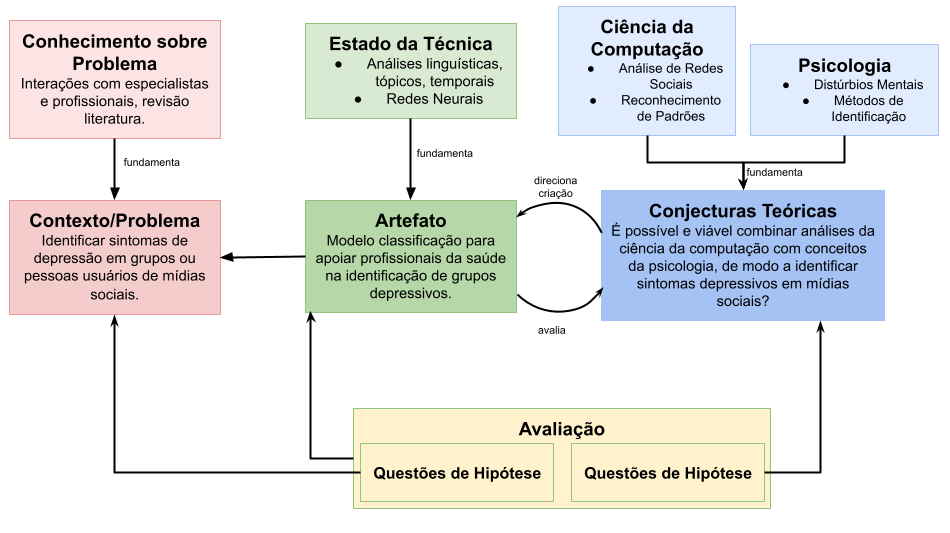
\includegraphics[scale=.4]{Graphics/Instancia DSR.png}
    \caption{Instanciação baseada no modelo de \cite{Pimentel2020}.}
  \end{figure}
\end{frame}

% \begin{frame}{Avaliações para }
  
% \end{frame}


% {\1
% \begin{frame}[plain,noframenumbering]
%   \finalpage{Thank you for using Feather Beamer Theme!}
% \end{frame}}
\begin{frame}{Bibliografia}
  \frametitle{Bibliografia}
  \bibliographystyle{apalike}
  \bibliography{bibliografia.bib}
  
\end{frame}

\end{document}